\documentclass[11pt,aspectratio=43]{beamer}
\usepackage[utf8]{inputenc}
\usepackage{amsmath, amsfonts, amssymb, amsthm}
\usepackage[T1]{fontenc}
\usepackage{lmodern}
\usepackage{xcolor}
\usepackage{setspace}
\usepackage{booktabs}
\usepackage{multirow}
\usepackage{graphicx}
\usepackage{tikz}
% \usetikzlibrary{decorations}
\usetikzlibrary{decorations.pathreplacing}
\usepackage{ulem}
\usepackage{hyperref}
\usepackage{booktabs}
\usepackage{babel}
\usepackage{makecell}
\usepackage[para,online,flushleft]{threeparttable}
\usepackage{pdfpages}
\usepackage{tcolorbox}
\usepackage{bm}
\usepackage{appendixnumberbeamer}
\usepackage{natbib}
\usepackage{caption}
\captionsetup[figure]{labelformat=empty}% redefines the caption setup of the figures environment in the beamer class.
\usetheme[compress]{Boadilla}
\usecolortheme{default}
\useoutertheme{miniframes}
\usefonttheme[onlymath]{serif}

\newcommand{\jump}[2]{\hyperlink{#1}{\beamerbutton{#2}}}
\newcommand{\orange}[1]{\textcolor{orange}{#1}}
\newcommand{\red}[1]{\textcolor{red}{#1}}

\setbeamertemplate{itemize item}{\raisebox{0.1em}{\scalebox{0.7}{$\blacksquare$}}}
\setbeamertemplate{itemize subitem}[circle]
\setbeamertemplate{itemize subsubitem}{--}
\setbeamercolor{itemize item}{fg=black}
\setbeamercolor{itemize subitem}{fg=black}
\setbeamercolor{itemize subsubitem}{fg=black}
\setbeamercolor{item projected}{bg=darkgray,fg=white}
\definecolor{blue}{rgb}{0.2, 0.2, 0.7}
\setbeamercolor{alerted text}{fg=blue}
\setbeamertemplate{enumerate items}[circle]


\setbeamertemplate{headline}{}

%==========================================
\let\olditemize=\itemize
\let\endolditemize=\enditemize
\renewenvironment{itemize}{\olditemize \itemsep1em}{\endolditemize}
\let\oldenumerate=\enumerate
\let\endoldenumerate=\endenumerate
\renewenvironment{enumerate}{\oldenumerate \itemsep1em}{ \endoldenumerate}

\DeclareMathOperator*{\argmax}{\arg\!\max}
\DeclareMathOperator*{\E}{\mathbb{E}}
\DeclareMathOperator*{\var}{\rm Var}
\DeclareMathOperator*{\cov}{\rm Cov}

\theoremstyle{definition}
\newtheorem{assume}{Assumption}
\newtheorem{lem}{Lemma}
\newtheorem{proposition}{Proposition}
\newtheorem{thm}{Theorem}
\newtheorem{corol}{Corollary}

\begin{document}
    \title[Lecture 10]{Lecture 10 \\ Examples on Competitive Equilibrium \\ and Social Planner's Problem}
    \author[Hui-Jun Chen]{Hui-Jun Chen}
    \institute[OSU]{The Ohio State University}
    % \date{\today}
    \date{\today}
    \setbeamertemplate{navigation symbols}{}
    \setstretch{1.2}

%-------------------------------------------------------
{
%	\usebackgroundtemplate{\includegraphics[width=1\paperwidth]{../EveningSky_cropped_edit43_bright.jpg}}
    \begin{frame}
% \vspace{3em}
        \centering
%		{\footnotesize 	ECON 4002 Intermediate Macroeconomic Theory}
        \maketitle
% \vspace{-1.5em}
% \centering
% \includegraphics[width=0.55\linewidth]{Pictures/houses.jpeg}


    \end{frame}
}

% -------------------------------------------
\setbeamertemplate{headline}
{
\setbeamercolor{section in head/foot}{fg=black, bg=white}
\vskip1em \tiny \insertsectionnavigationhorizontal{1\paperwidth}{\hspace{0.35\paperwidth}}{}
}
%------------------------------------------

\begin{frame}{Overview}
\label{slide:Overview}
    After constructing both \alert{consumers'} and \alert{firms'} problem, we start to bring them together in \alert{one-period model}:
    \begin{itemize}
        \item Lecture 8: \alert{competitive equilibrium} (CE)
        \begin{itemize}
            \item each agent solve their problems individually
            \item aggregate decision determines ``prices'' (wage, rent, etc.)
        \end{itemize}
        \item Lecture 9: \alert{social planer's problem} (SPP)
        \begin{itemize}
            \item imaginary and benevolent social planner determines the allocation
            \item should be the most efficient outcome
        \end{itemize}
        \item Lecture 10: CE and SPP examples
    \end{itemize}
\end{frame}

\section{Math Prepare}
\label{sec:Math_Prepare}

\begin{frame}{Two Dimensional Chain Rule}
\label{slide:Two_Dimensional_Chain_Rule}
    Suppose we have a utility function $ U( C, l ) $, where $ C $ is the consumption, and $ l $ is the leisure, and both $ C = C( w ) $ and $ l = l( w ) $ are the function of equilibrium wage $ w $, then
    %
    \begin{equation}
    \label{eq:chain_rule}
        \begin{split}
            \frac{d}{dw} [ U( C( w ), l( w ) ) ]
                & = D_{C}U( C( w ), l( w ) ) \times \frac{d C( w )}{d w}
            \\
                & \quad + D_{l} U( C( w ), l( w ) ) \times \frac{d l( w )}{dw}
            \\
        \end{split}
    \end{equation}
    %
\end{frame}

\begin{frame}{``Taken as Given''}
\label{slide:__Taken_as_Given}

Here is a good rule of thumb:
\begin{center}
    When you solve the problem of an agent who \alert{chooses $ y $} \red{taking $ x $ as given}, the answer should take the form of $ \alert{y}( \red{x} ) $.
\end{center}
\textbf{Example}: the consumer maximizes utility by \alert{choosing consumption, leisure, and labor supply}, \red{taking the wage and profits as given}. ($G = 0$)
%
\begin{equation}
\label{eq:taken_as_given}
    \max_{\alert{C, l, N^{s}}} U( C, l ) \quad \text{subject to} \quad C = \red{w} N^{s} + \red{\pi} \quad \text{and} \quad l + N^{s} = h
\end{equation}
%
\begin{itemize}
    \item solution takes the form: $ \alert{C}( \red{w, \pi} ), \alert{l}( \red{w, \pi} ), \alert{N^{s}}( \red{w, \pi} )$
    \item why not $ h $, or utility parameters? Not \textbf{endogenous to the model!}
    \item can repeat this idea for the firm to get $ \alert{N^{d}}( \red{w} ), \alert{Y}( \red{w} ), \alert{\pi}( \red{w} )$
\end{itemize}
\end{frame}

\begin{frame}{``Endogenous to the Model''}
\label{slide:__Endogenous_to_the_Model__}
    What does equilibrium do? Figures out what level of ``taken as given'' but endogenous variables has to occur:
    \begin{itemize}
        \item consumer: $ \pi = \pi( w ) $ from firm's problem
        \item labor supply can be rewrite as: $ N^{s} ( w, \pi ) = N^{s}( w, \pi( w ) ) = N^{s}( w )$
        \item labor market clearing: $ N^{d}( w^{*} ) = N^{s}( w^{*} ) $, where $ w^{*} $ is eqm wage
    \end{itemize}
    \textbf{Question}: any of the ``taken as given variables'' show up in the SPP?
    \begin{itemize}
        \item Ans: NO! Social planner is \alert{benevolent dictator}!
    \end{itemize}
\end{frame}

\section{Environment}
\label{sec:Environment}

\begin{frame}{Model Environment}
\label{slide:Model_Environment}
    \begin{itemize}
        \item Consumer: $ U( C, l ) = \frac{C^{1-b}}{1-b} + \frac{l^{1-d}}{1-d} $, where $ b=2 $ and $ d = \frac{3}{2} $.
        \begin{itemize}
            \item $ b, d $ are \alert{parameters}
            \item $ h = 1 $ is time endowment to allocate between leisure and labor supply
            \item owns the firm, subject to lump-sum tax $ T \ge  0 $
        \end{itemize}
        \item Firm: $ z F( K, N ) = z K^{\alpha} N^{1-\alpha} $, where $ K = 1 $ and $ \alpha = \frac{1}{2} $ (param)
        \item Government: $ T = G $
        \item Labor market: both consumer and firm take wage rate $ w $ as given
    \end{itemize}
\end{frame}

\begin{frame}{Experiments}
\label{slide:Experiments}
    \begin{enumerate}
        \item \textbf{Benchmark}: $ z = 1 $ and $ G = 0 $
        \item \textbf{Experiment 1}: $ \alert{z = 1.2} $ and $ G = 0 $
        \item \textbf{Experiment 2}: $ z = 1 $ and $ G = 0.5 $
    \end{enumerate}
\end{frame}

\section{Benchmark}
\label{sec:Benchmark}

\begin{frame}{Solve Benchmark in Social Planner's Problem}
\label{slide:Solve_Benchmark_in_Social_Planner_s_Problem}
    \begin{itemize}
        \item PPF: $ C + G = z N^{1-\alpha} $, where $ \alpha = \frac{1}{2} $
        \item Time: $ N = h - l $, where $ h = 1 $
        \item Social Planner's Problem:
        %
        \begin{equation}
        \label{eq:SPP_Benchmark}
            \begin{split}
                \max_{l} \quad
                    & U( C( l ), l ) = \frac{C( l )^{1-b}}{1-b} + \frac{l^{1-d}}{1-d}
                \\
                \text{s.t.} \quad
                    & C = Y - G
                \\
                    & Y = z N^{1-\alpha}
                \\
                    & N = 1 - l
                \\
                \Rightarrow \quad \max_{l} \quad
                    & \frac{(z ( 1-l )^{1-\alpha} - G)^{1-b}}{1-b} + \frac{l^{1-d}}{1-d}
                \\
            \end{split}
        \end{equation}
        %
    \end{itemize}
\end{frame}

\begin{frame}{Solve Benchmark in Social Planner's Problem (Cont.)}
\label{slide:Solve_Benchmark_in_Social_Planner_s_Problem__Cont__}
\begin{align}
        & \max_{l} \quad \frac{(z ( 1-l )^{1-\alpha} - G)^{1-b}}{1-b} + \frac{l^{1-d}}{1-d}
    \\
    \text{FOC:} \quad
        & \scriptsize
            \underbrace{( z ( 1-l )^{1-\alpha} - G )^{-b}}_{ \frac{( \cdot )^{1-b}}{1-b}}
            \times \underbrace{( 1-\alpha )z( 1-l )^{-\alpha}}_{ z( 1-l )^{1-\alpha}}
            \times \underbrace{( -1 )}_{-l}
            + l^{-d} = 0
    \\
    G = 0 : \quad
        & \scriptsize
            z^{-b}( 1-l )^{-b(1-\alpha)} \times ( 1-\alpha ) z( 1-l )^{-\alpha} = l^{-d}
    \\
        & \scriptsize
            ( 1-\alpha ) z^{1-b} ( 1-l )^{-\alpha - b+ \alpha b} = l^{-d}
    \\
        & \scriptsize
            \alpha = 1/2; \quad b = 2; \quad d = 3/2
    \\
    \text{Apply:} \quad
        & \scriptsize
            \frac{1}{2} z^{-1} ( 1-l )^{-\frac{3}{2}} = l^{-\frac{3}{2}} \Rightarrow  \frac{1}{2z} = ( \frac{1-l}{l} )^{ \frac{3}{2}}
    \\
        & \scriptsize
            \Rightarrow \frac{1-l}{l} = ( \frac{1}{2z} )^{\frac{2}{3}} \Rightarrow l( z, 0 ) = \frac{1}{1 + (2z)^{-\frac{2}{3}}}
    \\
    z = 1 \quad
        & \scriptsize
            \Rightarrow l \approx 0.61, N \approx 0.39, Y = C \approx 0.62, w = \frac{z}{2} N^{-\frac{1}{2}} \approx 0.8
\end{align}
\end{frame}

\begin{frame}{Visualization: Benchmark in SPP}
\label{slide:Visualization__Benchmark_in_SPP}
    \begin{columns}
        \begin{column}{0.5\textwidth}
            \begin{figure}
                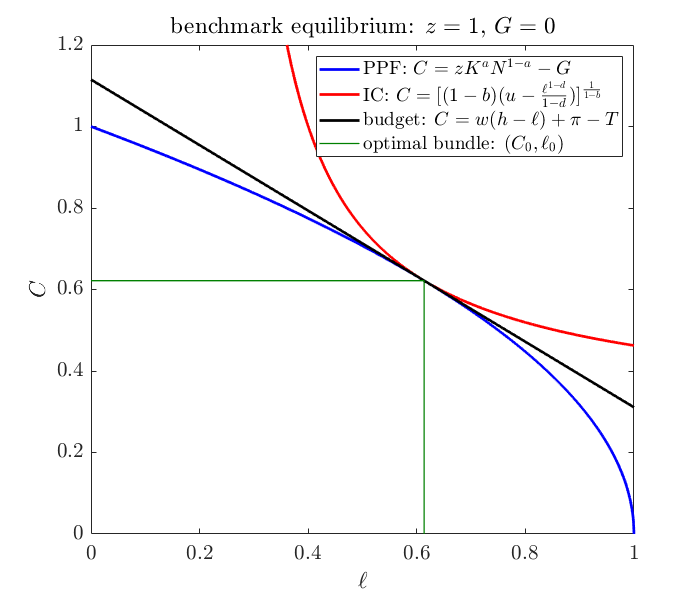
\includegraphics[width=\textwidth]{./figures/benchmark.png}
            \end{figure}
        \end{column}
        \begin{column}{0.5\textwidth}
            Indifference curve and PPF are tangent at optimal bundle
            %
            \begin{align*}
                    & \text{slope at tangency } ( C_{0}, l_{0} )
                \\
                = \quad
                    & \text{slope of IC} (-MRS_{l, C})
                \\
                = \quad
                    & \text{slope of budget line} (-w)
                \\
                = \quad
                    & \text{slope of PPF} (-MRT_{l, C})
                \\
                = \quad
                    & \text{slope of production fcn} (-MPN)
            \end{align*}
            %
        \end{column}
    \end{columns}
\end{frame}

\section{Experiments}
\label{sec:Experiments}

\begin{frame}{Solving with New TFP}
\label{slide:Solving_with_New_TFP}
    \begin{columns}
        \begin{column}{0.5\textwidth}
            \begin{figure}
                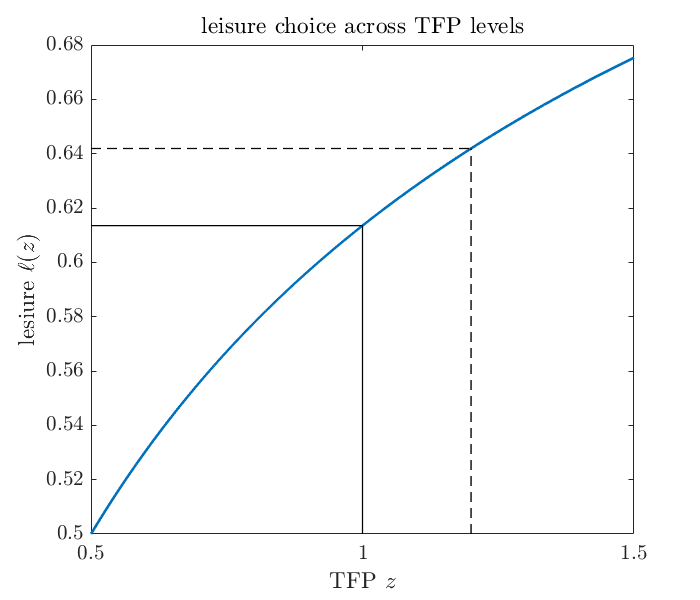
\includegraphics[width=\textwidth]{./figures/TFPsolveSPP.png}
            \end{figure}
        \end{column}
        \begin{column}{0.5\textwidth}
            Recall that we solved for the equilibrium quantity of leisure as a function of TFP:
            %
            \begin{equation}
            \label{eq:leisure}
                l( z ) = \frac{1}{1 + ( 2z )^{-\frac{2}{3}}}
            \end{equation}
            %
            So now we’ve solved for all possible ``experiment 1’s''! Just plug in $ z = 1.2 $ to get $ l \approx 0.642 $, and plug in to get all the rest as well.
        \end{column}
    \end{columns}
\end{frame}

\begin{frame}{Visualization: Experiment 1}
\label{slide:Visualization__Experiment_1}
    \begin{columns}
        \begin{column}{0.5\textwidth}
            \begin{figure}
                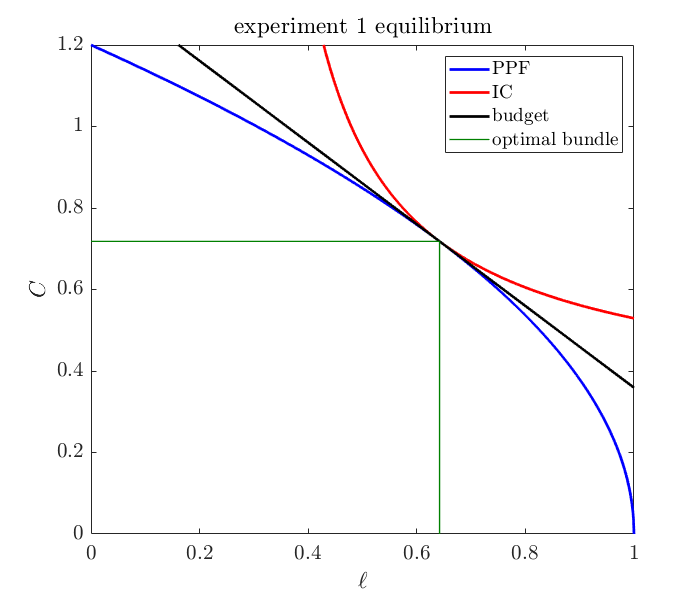
\includegraphics[width=\textwidth]{./figures/Exp1.png}
            \end{figure}
        \end{column}
        \begin{column}{0.5\textwidth}
            Tangency preserved, just \alert{shifted}
            %
            \begin{align*}
                    & \text{slope at tangency } \alert{( C_{1}, l_{1} )}
                \\
                = \quad
                    & \text{slope of IC} (-MRS_{l, C})
                \\
                = \quad
                    & \text{slope of budget line} (-w)
                \\
                = \quad
                    & \text{slope of PPF} (-MRT_{l, C})
                \\
                = \quad
                    & \text{slope of production fcn} (-MPN)
            \end{align*}
            %
        \end{column}
    \end{columns}
\end{frame}


\begin{frame}{Comparison: Experiment 1 and Benchmark}
\label{slide:Comparison__Experiment_1_and_Benchmark}
\begin{columns}
    \begin{column}{0.5\textwidth}
        \begin{figure}
            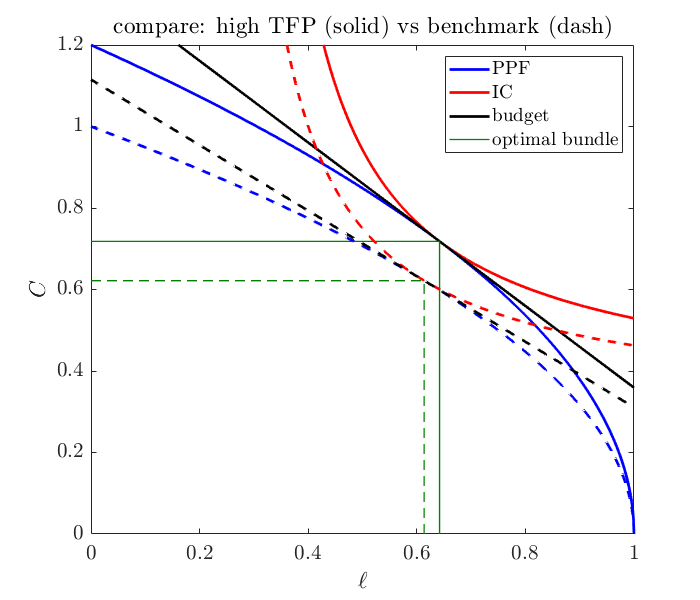
\includegraphics[width=\textwidth]{./figures/Exp1BenchmarkCompare.png}
        \end{figure}
    \end{column}
    \begin{column}{0.5\textwidth}
        What’s different?
        \begin{itemize}
            \item higher productivity means PPF shifts outward
            \item outward shift of PPF makes higher utility level (IC) attainable
            \item tangency is steeper: wage increases
            \item both consumption and leisure increase!
        \end{itemize}
    \end{column}
\end{columns}
\end{frame}

\begin{frame}{Experiment 1: Income and Substitution Effect}
\label{slide:Experiment_1__Income_and_Substitution_Effect}
    \begin{columns}
        \begin{column}{0.5\textwidth}
            \begin{figure}
                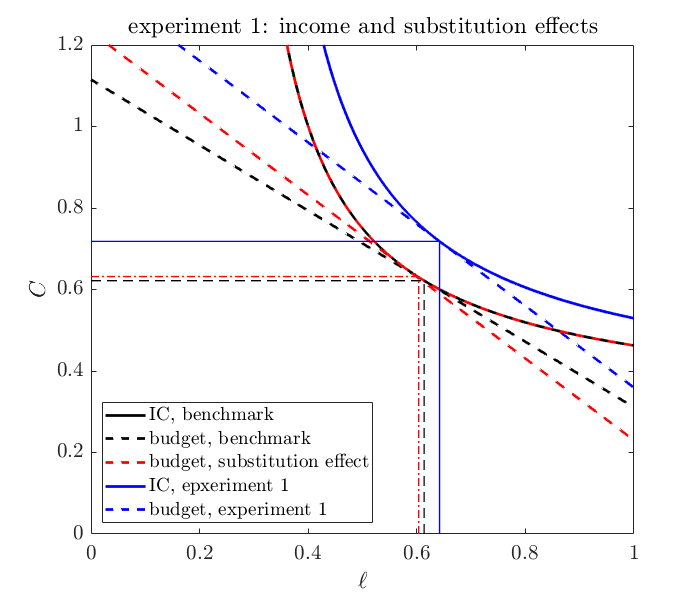
\includegraphics[width=\textwidth]{./figures/IncomeSubEffect.png}
            \end{figure}
        \end{column}
        \begin{column}{0.5\textwidth}
            Recall wage increase case from the consumer problem:
            \begin{itemize}
                \item \textbf{substitution effect:} move along IC but reflect new wage (i,e, new budget or new PPF)
                \begin{itemize}
                    \item $ C $ increases, $ l $ decreases
                \end{itemize}
                \item \textbf{income effect:} move up to new budget line / PPF
                \begin{itemize}
                    \item $ C $ and $ l $ both increase
                \end{itemize}
                \item here, income effect wins and leisure increases
            \end{itemize}
        \end{column}
    \end{columns}
\end{frame}

\begin{frame}{Comparison: Experiment 2 and Benchmark}
\label{slide:Comparison__Experiment_2_and_Benchmark}
    \begin{columns}
        \begin{column}{0.5\textwidth}
            \begin{figure}
                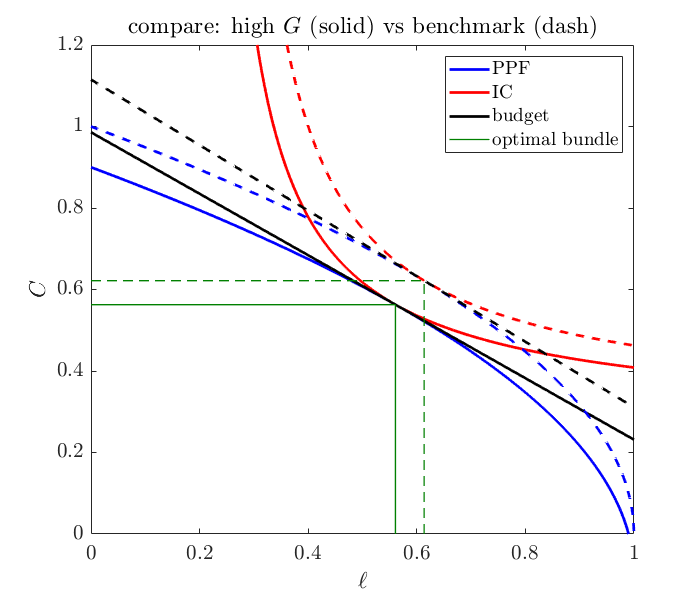
\includegraphics[width=\textwidth]{./figures/Exp2BenchmarkCompare.png}
            \end{figure}
        \end{column}
        \begin{column}{0.5\textwidth}
            Note: SPP harder to solve by hand with $ G \neq 0$ \jump{slide:How_to_solve___G__neq_0__}{details}.
            But, can still analyze with graphs!
            \begin{itemize}
                \item higher government spending shifts PPF \alert{inward}
                \item inward shift of PPF lowers utility level (IC) attainable
                \item budget shallower: wage falls
                \item consumption, leisure fall (recall normal goods assumption)
                \item can show output increases
            \end{itemize}
        \end{column}
    \end{columns}
\end{frame}

\section{Summary}
\label{sec:Summary}

\begin{frame}{Response to Data}
\label{slide:Response_to_Data}
    \begin{columns}
        \begin{column}{0.7\textwidth}
            \begin{tabular}{l|l|l}
                Effect of $\uparrow$ in & TFP       & G        \\
                \hline
                \hline
                Output                  & Increase  & Increase \\
                \hline
                Consumption             & Increase  & Decrease \\
                \hline
                Employment              & Ambiguous & Increase \\
                \hline
                Wage                    & Increase  & Decrease
            \end{tabular}
        \end{column}
        \begin{column}{0.3\textwidth}
            TFP is a overall better match!
            \alert{Real Business Cycle} theory
        \end{column}
    \end{columns}
    \begin{itemize}
        \item recall key \alert{business cycle facts}: employment, consumption, real wage are all procyclical
        \item recall key \alert{trend}: output has grown steadily for last century
        \item question: which model is more consistent with these facts?
    \end{itemize}
\end{frame}

\begin{frame}{Data: Government Spending from WWII}
\label{slide:Data__Government_Spending_from_WWII}
    \begin{columns}
        \begin{column}{0.5\textwidth}
            \begin{figure}
                \caption{\scriptsize Figure 5.7  GDP, Consumption, and Government Expenditures}
                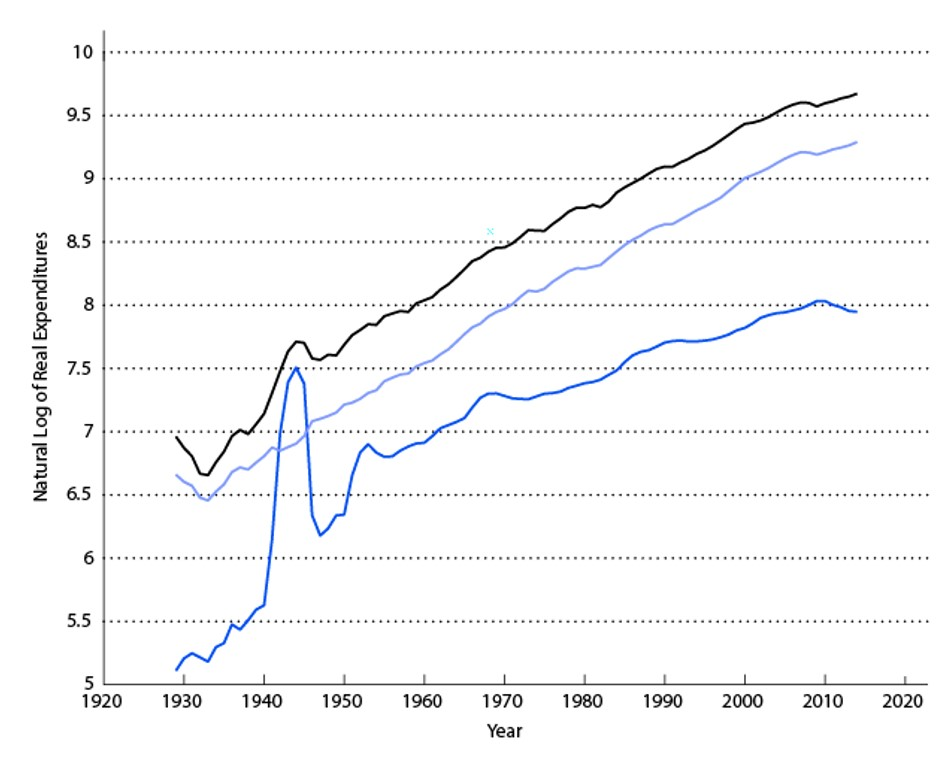
\includegraphics[width=\textwidth]{./figures/Figure5_7.jpg}
            \end{figure}
        \end{column}
        \begin{column}{0.5\textwidth}
            \begin{itemize}
                \item large increase in $ G $ to finance war effort
                \item modest increase in $ Y $
                \item slight decline in $ C $
                \item consistent with our model!
            \end{itemize}
        \end{column}
    \end{columns}
\end{frame}

\begin{frame}{Data: Solow Residual, $ z = \frac{Y}{K^{\alpha} N^{1-\alpha}} $}
\label{slide:Data__Solow_Residual____z____frac_Y__K___alpha__N__1__alpha____}
    \begin{columns}
        \begin{column}{0.5\textwidth}
            \begin{figure}
                \caption{\scriptsize Figure 4.18  The Solow Residual for the United States}
                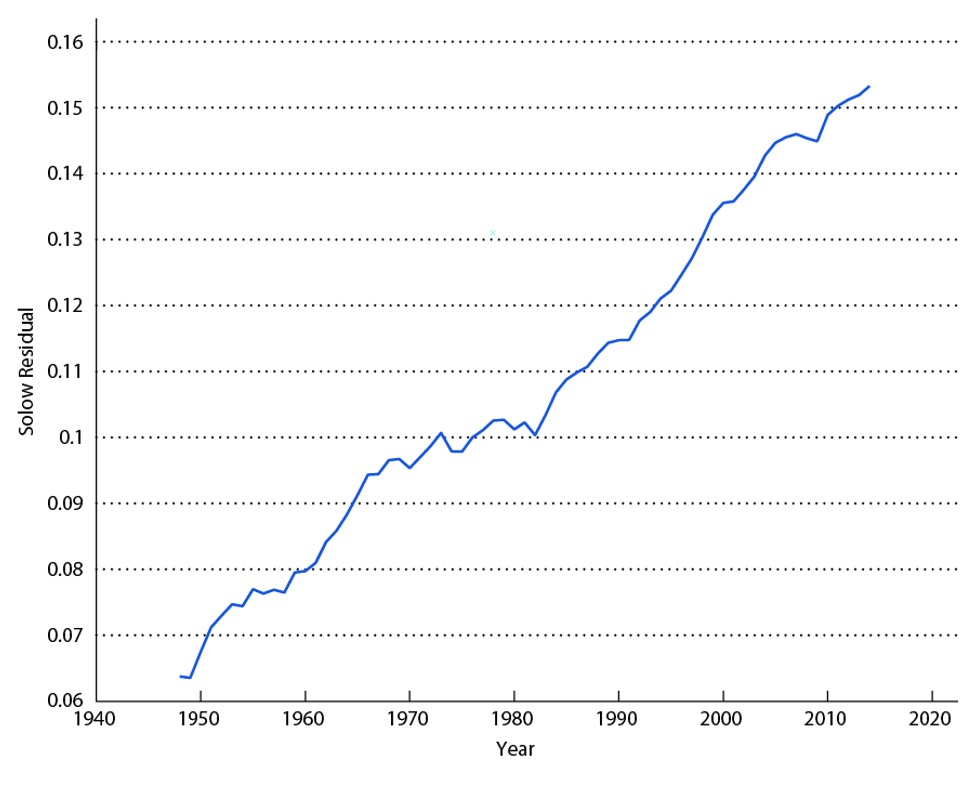
\includegraphics[width=\textwidth]{./figures/Figure4_18.jpg}
            \end{figure}
        \end{column}
        \begin{column}{0.5\textwidth}
            \begin{figure}
                \caption{\scriptsize Figure 5.11  Deviations from Trend in GDP and the Solow Residual}
                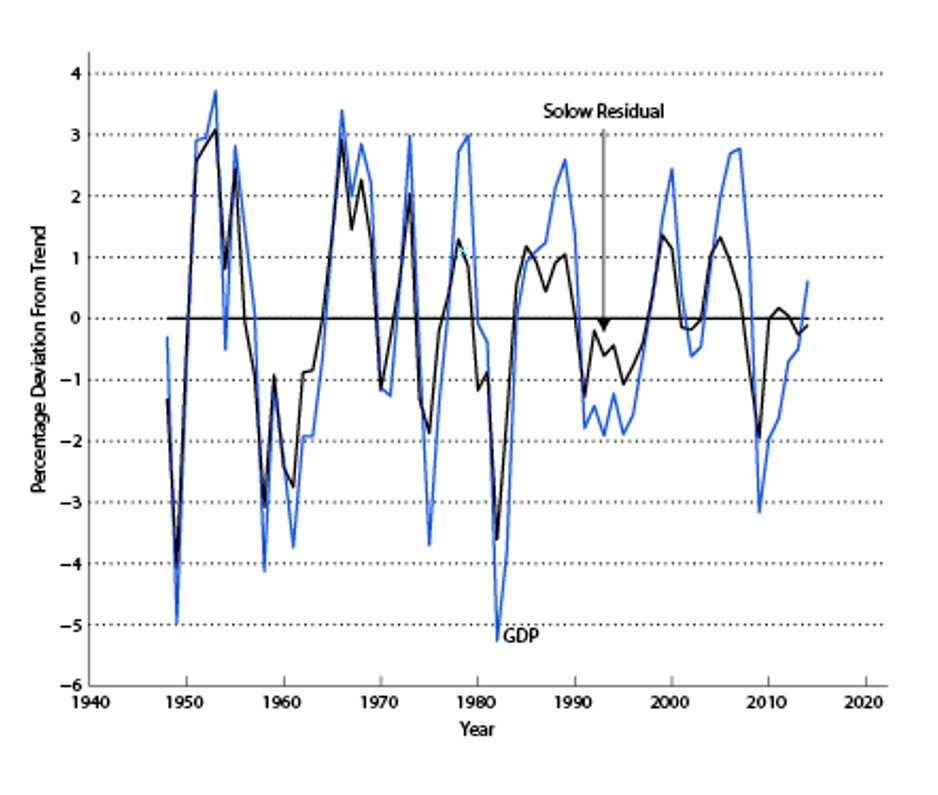
\includegraphics[width=\textwidth]{./figures/Figure5_11.jpg}
            \end{figure}
        \end{column}
    \end{columns}
\end{frame}





\section{Appendix}
\label{sec:Appendix}

\appendix
% -------------------------------------------
\setbeamertemplate{headline}
{
\setbeamercolor{section in head/foot}{fg=black, bg=white}
\vskip1em \tiny \insertsectionnavigationhorizontal{1\paperwidth}{\hspace{0.50\paperwidth}}{}
}
%------------------------------------------
\begin{frame}\frametitle{}
\begin{columns}
\label{Appendix}
\column{1\linewidth}
\centering
{\Large \alert{Appendix}}
\end{columns}
\end{frame}
%------------------------------------------
\begin{frame}{How to solve $ G \neq 0 $}
\label{slide:How_to_solve___G__neq_0__}
\framesubtitle{\jump{slide:Comparison__Experiment_2_and_Benchmark}{Back}}
\begin{align}
        & \max_{l} \quad \frac{(z ( 1-l )^{1-\alpha} - G)^{1-b}}{1-b} + \frac{l^{1-d}}{1-d}
    \\
    \text{FOC:} \quad
        & \scriptsize
            z ( 1-l )^{1-\alpha} - G )^{-b}
            \times ( 1-\alpha )z( 1-l )^{-\alpha}
            = l^{-d}
    \\
    \text{Divide}: \quad
        & ( z ( 1-l )^{1-\alpha} - G )^{-b} = \frac{l^{-d}}{( 1-\alpha )z( 1-l )^{-\alpha}}
    \\
    \text{power of } -\frac{1}{b}: \quad
        & z ( 1-l )^{1-\alpha} - G =
            \left[
                \frac{l^{-d}}{( 1-\alpha )z( 1-l )^{-\alpha}}
            \right]^{-\frac{1}{b}}
    \\
    \text{Solve } G: \quad
        & G = F( l ) = z( 1-l )^{1-\alpha} -
            \left[
                \frac{l^{-d}}{( 1-\alpha )z( 1-l )^{-\alpha}}
            \right]^{-\frac{1}{b}}
    \\
        & \iff l = F^{-1}( G )
\end{align}
\end{frame}

\end{document}

